%%%%%%%%%%%%%%%%%%%%%%%%%%%%%%%%%%%%%%%%%
% Beamer Presentation
% LaTeX Template
% Version 1.0 (10/11/12)
%
% This template has been downloaded from:
% http://www.LaTeXTemplates.com
%
% License:
% CC BY-NC-SA 3.0 (http://creativecommons.org/licenses/by-nc-sa/3.0/)
%
%%%%%%%%%%%%%%%%%%%%%%%%%%%%%%%%%%%%%%%%%

%----------------------------------------------------------------------------------------
%	PACKAGES AND THEMES
%----------------------------------------------------------------------------------------

\documentclass{beamer}

\mode<presentation> {

% The Beamer class comes with a number of default slide themes
% which change the colors and layouts of slides. Below this is a list
% of all the themes, uncomment each in turn to see what they look like.

%\usetheme{default}
%\usetheme{AnnArbor}
%\usetheme{Antibes}
%\usetheme{Bergen}
%\usetheme{Berkeley}
%\usetheme{Berlin}
%\usetheme{Boadilla}
%\usetheme{CambridgeUS}
%\usetheme{Copenhagen}
%\usetheme{Darmstadt}
%\usetheme{Dresden}
%\usetheme{Frankfurt}
%\usetheme{Goettingen}
%\usetheme{Hannover}
%\usetheme{Ilmenau}
%\usetheme{JuanLesPins}
%\usetheme{Luebeck}
\usetheme{Madrid}
%\usetheme{Malmoe}
%\usetheme{Marburg}
%\usetheme{Montpellier}
%\usetheme{PaloAlto}
%\usetheme{Pittsburgh}
%\usetheme{Rochester}
%\usetheme{Singapore}
%\usetheme{Szeged}
%\usetheme{Warsaw}

% As well as themes, the Beamer class has a number of color themes
% for any slide theme. Uncomment each of these in turn to see how it
% changes the colors of your current slide theme.

%\usecolortheme{albatross}
%\usecolortheme{beaver}
%\usecolortheme{beetle}
%\usecolortheme{crane}
%\usecolortheme{dolphin}
%\usecolortheme{dove}
%\usecolortheme{fly}
%\usecolortheme{lily}
%\usecolortheme{orchid}
%\usecolortheme{rose}
%\usecolortheme{seagull}
%\usecolortheme{seahorse}
%\usecolortheme{whale}
%\usecolortheme{wolverine}

%\setbeamertemplate{footline} % To remove the footer line in all slides uncomment this line
%\setbeamertemplate{footline}[page number] % To replace the footer line in all slides with a simple slide count uncomment this line

%\setbeamertemplate{navigation symbols}{} % To remove the navigation symbols from the bottom of all slides uncomment this line
}

\usepackage{graphicx} % Allows including images
\usepackage{booktabs} % Allows the use of \toprule, \midrule and \bottomrule in tables

%----------------------------------------------------------------------------------------
%	TITLE PAGE
%----------------------------------------------------------------------------------------

\title[Classifications of systems]{Classifications of systems} % The short title appears at the bottom of every slide, the full title is only on the title page

\author{} % Your name
\institute[KU Leuven] % Your institution as it will appear on the bottom of every slide, may be shorthand to save space
{
Katholieke Universiteit Leuven \\ % Your institution for the title page
\medskip
\textit{} % Your email address
}
\date{\today} % Date, can be changed to a custom date

\begin{document}

\begin{frame}
\titlepage % Print the title page as the first slide
\end{frame}

\begin{frame}
\frametitle{Overview} % Table of contents slide, comment this block out to remove it
\tableofcontents % Throughout your presentation, if you choose to use \section{} and \subsection{} commands, these will automatically be printed on this slide as an overview of your presentation
\end{frame}

%----------------------------------------------------------------------------------------
%	PRESENTATION SLIDES
%----------------------------------------------------------------------------------------

%------------------------------------------------
\section{Number of inputs and outputs} 
%------------------------------------------------

\begin{frame}
\frametitle{Based on the number of inputs and outputs}
\begin{enumerate}
\item \textbf{SISO}: Single Input Single Output
\item \textbf{SIMO}: Single Input Multiple Output
\item \textbf{MISO}: Multiple Input Single Output
\item \textbf{MIMO}: Multiple Input Multiple Output
\item \textbf{Autonomous}: No inputs and one or more outputs
\end{enumerate}
\end{frame}

%------------------------------------------------
\section{Continuous vs. Discrete time} 
%------------------------------------------------

\begin{frame}
\frametitle{Continuous vs. Discrete time}
We will discuss both types simultaneously in order to emphasize the similarities (and differences).\\
\medskip
\begin{columns}[c] 

\column{.5\textwidth}
\center \textbf{Continuous system}
\begin{enumerate}
\item It has continuous input and output signals
\item We denote continuous time by $t \in \Re$
\item We denote functions of continuous time with round brackets, e.g.: $x(t)$
\end{enumerate}

\column{.5\textwidth}
\center \textbf{Discrete system}
\begin{enumerate}
\item It has discrete input and output signals
\item We denote discrete time by $k \in Z$
\item We denote functions of continuous time with square brackets, e.g.: $x[k]$
\end{enumerate}

\end{columns}
\end{frame}

%------------------------------------------------

\begin{frame}
\frametitle{Continuous vs. Discrete time}
\begin{columns}[c] 

\column{.5\textwidth}
\center {\textbf{Continuous}}\\
For every moments $t \in \Re$, the system has: 
\begin{enumerate}
\item A vector of inputs \textbf{u}(t)
\item A vector of outputs \textbf{y}(t)
\item A vector of states \textbf{x}(t)
\end{enumerate}
\begin{figure}
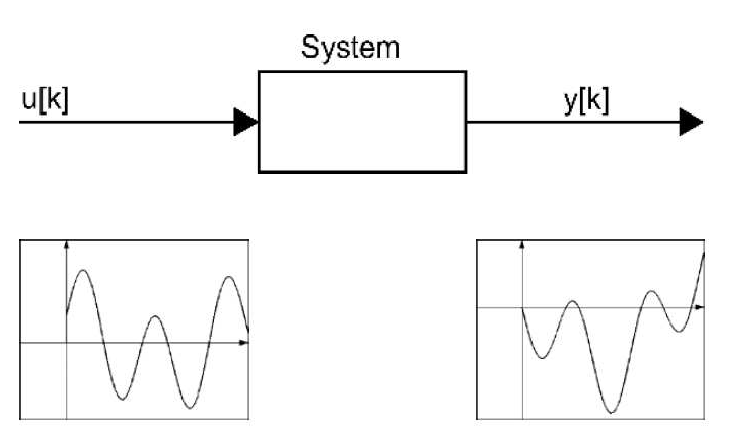
\includegraphics[width=0.8\linewidth]{continuous}
\end{figure}

\column{.5\textwidth}
\center {\textbf{Discrete}}\\
For every moments $k \in Z$, the system has: 
\begin{enumerate}
\item A vector of inputs \textbf{u}[k]
\item A vector of outputs \textbf{y}[k]
\item A vector of states \textbf{x}[k]
\end{enumerate}
\begin{figure}
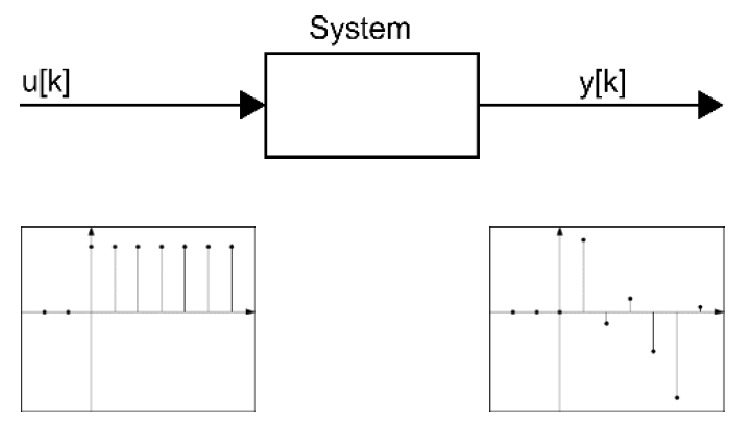
\includegraphics[width=0.8\linewidth]{discrete}
\end{figure}

\end{columns}
\end{frame}

%------------------------------------------------
\section{Linear vs. Nonlinear}
%------------------------------------------------

\begin{frame}
\frametitle{}
\end{frame}

%------------------------------------------------
\section{Causal vs. Non-causal} 
%------------------------------------------------

\begin{frame}
\frametitle{}
\end{frame}

%------------------------------------------------
\section{Time-invariant vs. Time-varying} 
%------------------------------------------------

\begin{frame}
\frametitle{}
\end{frame}

%------------------------------------------------
\section{Lumped vs. Distributed} 
%------------------------------------------------

\begin{frame}
\frametitle{}
\end{frame}

%----------------------------------------------------------------------------------------

\end{document} 